% -*- coding: utf-8 -*-

\documentclass[UTF8]{ctexart} %ctexart 中文tex类型 默认每段自动锁紧两个字符,英文段首缩进4个字符
\usepackage{graphicx} %graphicx宏包可以使用命令 
\usepackage{listings} 
\usepackage{shapepar}
\usepackage{float}
\title{标题:First LaTeX}
\author{作者:Monburan}
\date{创建日期:\today}

\begin{document}

\maketitle

\begin{abstract}
% abstractname 用来设置摘要的文字
简单体验 \LaTeX\ ,创建这个文件的目的是引导初学者了解 \LaTeX\ 基本语法,如果想深入学习请购买《LaTeX入门》等专业书籍。
\end{abstract}
\noindent
最基本中英文字排版展示:

This is my document. This is my document. This is my document. This is my document.

power by \LaTeX\ ! power by \LaTeX\ ! power by \LaTeX\ ! power by \LaTeX\ !

这是我的文档。这是我的文档。这是我的文档。这是我的文档。

使用 \LaTeX\ 强力驱动! 使用 \LaTeX\ 强力驱动! 使用 \LaTeX\ 强力驱动! 使用 \LaTeX\ 强力驱动!

\noindent
如果你觉得这个太无聊 \LaTeX\ 还可以这样玩:

\heartpar{
    love       you
  someone ! I love you !
  someone ! I love you !
  someone ! I love you !
  someone ! I love you !
  someone ! I love you !
  someone ! I love you !
  someone ! I love you !
  someone ! I love you !
}

\noindent
尝试插入表格:

\noindent %不使用首行缩进
\begin{tabular}{|rrr|}

\hline
第 $a$ 列 & 第 $b$ 列 & 第 $c$ 列 \\
\hline
1 & 3 & 5 \\
2 & 4 & 6 \\
\hline
\end{tabular}

有序列表:

\begin{enumerate}
 \item 中文
 \item English
 \item ...
\end{enumerate}

无序列表:

\begin{itemize}
 \item 中文
 \item English
 \item ...
\end{itemize}

有条目关键字的列表:

\begin{description}
 \item[中文] 中国使用的文字
 \item[English] 英国为首的欧美国家使用的文字
 \item[其他] 其他文字
\end{description}

尝试插入代码:

\begin{verbatim}
# -*- coding: UTF-8 -*-
name = Jack
def return_name(name):
    if name:
        return name
    if not name:
        return 'who are you?'
\end{verbatim}

虽然上面的代码格式已经足够美观了,\LaTeX\ 依旧可以做到更好,下面尝试对上面的代码片段进行美化,并在其中加入汉字注释:
\lstset{
 basicstyle=\sffamily,
 keywordstyle=\bfseries,
 commentstyle=\rmfamily\itshape,
 stringstyle=\ttfamily,
 columns=flexible,
 numbers=left,
 numberstyle=\footnotesize,
 escapechar=`
 }
\begin{lstlisting}[language=Python]
# -*- coding: UTF-8 -*-
name = Jack
def return_name(name):
    # `你看中文注释就这样出现了`
    if name:
        return name
    if not name:
      return 'who are you?'

\end{lstlisting}

\begin{figure}[H] %插图使用不浮动环境
\centering
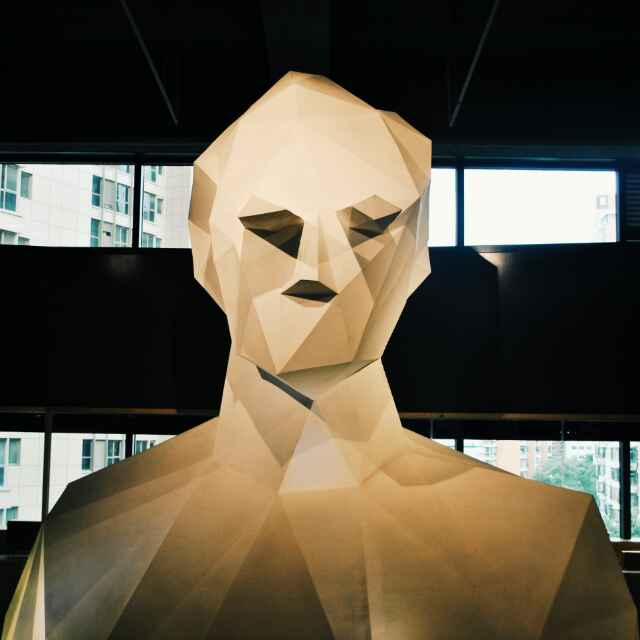
\includegraphics[scale=0.3]{webwxgeticon.jpg} % \includegraphics 插入图片
\caption{这是我的头像}
\label{fig:xiaotu}
\end{figure}
\end{document}